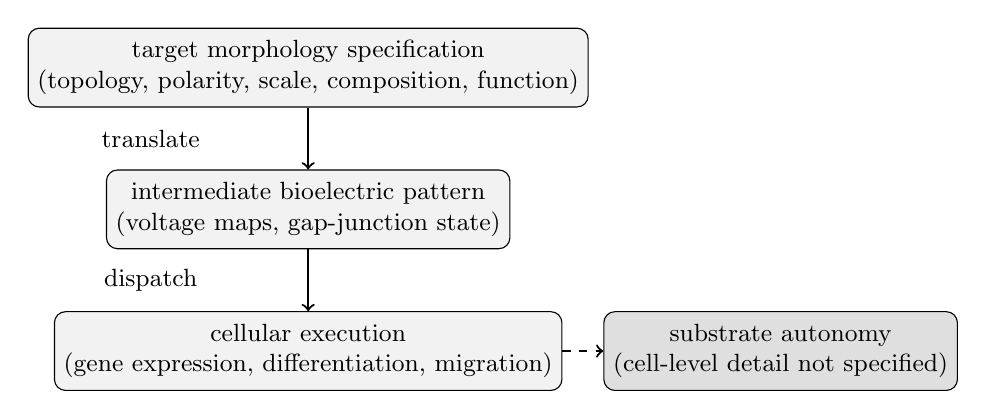
\begin{tikzpicture}[x=1cm, y=0.9cm, font=\small,
    box/.style={draw, rounded corners, minimum width=4cm, minimum height=1cm,
      align=center, fill=gray!10},
    arrow/.style={->, thick}]
  \node[box] (spec) at (4, 5) {target morphology specification\\
    (topology, polarity, scale, composition, function)};
  \node[box] (pat) at (4, 3) {intermediate bioelectric pattern\\
    (voltage maps, gap-junction state)};
  \node[box] (cell) at (4, 1) {cellular execution\\
    (gene expression, differentiation, migration)};
  \node[box, fill=gray!25] (sub) at (10, 1) {substrate autonomy\\
    (cell-level detail not specified)};
  \draw[arrow] (spec) -- (pat);
  \draw[arrow] (pat) -- (cell);
  \draw[arrow, dashed] (cell) -- (sub);
  \node[align=center] at (2, 4) {translate};
  \node[align=center] at (2, 2) {dispatch};
\end{tikzpicture}
